\chapter{Il flusso unidirezionale con Flux e Redux}
E' stato spiegato come MVC gestisce la problematica del flusso dei dati attraverso la bidirezionalità, e tutti i problemi che quest'ultima causa nell'implementazione di una applicazione web complessa. Solo recentemente è stato implementato un nuovo tipo di approccio che cerca di ovviare a tutto ciò, ed è quello del “flusso unidirezionale”. Due sono le architetture che verranno analizzate: Flux e Redux, entrambe riescono a mantenere un alto livello di scalabilità a prescindere dalla complessità dell'applicazione e risolvono tutti i problemi legati al flusso bidirezionale ed MVC.

\section{Architettura Flux}
Flux è un'architettura recente creata da Facebook che struttura il front-end di una applicazione in modo che il flusso dei dati dall'innesco di un evento fino alle sue ripercussioni nell'interfaccia segua un'unica direzione.
Questo pattern, essendo molto astratto, non ha delle vere e proprie dipendenze ed è possibile applicarlo a qualsiasi tipo di applicazione con qualsivoglia linguaggio. E' tuttavia nato per strutturare applicazioni React e quindi perfezionato per tale libreria.

La struttura di tale paradigma si divide in quattro parti fondamentali: il \textit{Dispatcher}, gli \textit{Store}, le \textit{View} e le \textit{Action}.

\begin{figure}[h]
\centering
\vspace*{0.5cm} 
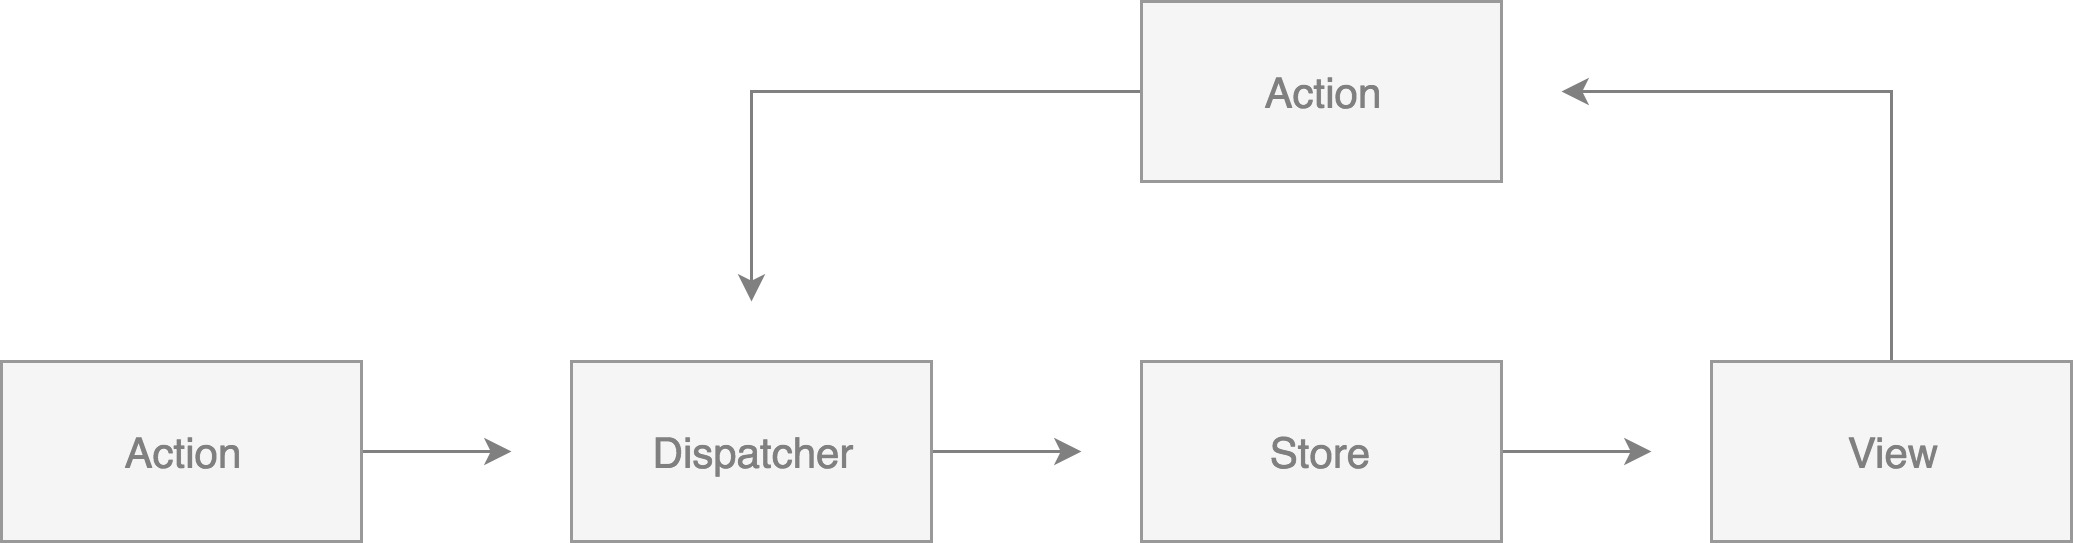
\includegraphics[width=14cm]{./images/FluxWorkflow}
\caption{Rappresentazione del flusso di dati con Flux.}
\label{FluxWorkflow}
\vspace*{0.5cm} 
\end{figure}

\noindent
In questa architettura la logica è divisa in due parti: ciò che riguarda gli eventi e le modifiche all'interfaccia è compreso nella View, la quale potrebbe essere definita una Controller-View in quanto esegue entrambi i lavori; la logica che riguarda invece lo stato dell'applicazione è compresa negli Store, i quali a seconda dell'azione eseguita si modificano di conseguenza.

\subsection{I componenti}
\label{FluxComponents}
Flux considera nella sua architettura quattro elementi fondamentali: Le \textit{Action}, il \textit{Dispatcher}, gli \textit{Stores} e le \textit{View}.

\subsubsection*{Action}
Le Action sono la moneta di scambio dell'architettura e vengono propagate dalle View (attraverso il Dispatcher) agli Store che le utilizzeranno per apportare modifiche a se stessi. Queste consistono generalmente in un oggetto composto da due elementi:

    \begin{itemize}
        \item \textbf{Nome}, che rappresenta lo scopo dell'azione da effettuare, ed è una stringa come ad esempio \mintinline{text}{AddArticle} o \mintinline{text}{RemoveUser}. 
        \item \textbf{Payload}, ossia l'insieme di dati necessari a portare a termine l'azione. Se si stesse parlando di una azione \mintinline{text}{AddArticle} ad esempio, il payload sarebbe composto dal titolo e dal contenuto dell'articolo da aggiungere.
    \end{itemize}

\noindent
Tutti gli eventi esistenti che modificano lo stato dell'applicazione devono essere descritti sotto forma di Action. In Flux qualsiasi cosa non sia un'azione non può verificarsi.

\subsubsection*{Dispatcher}
Il Dispatcher nell'architettura Flux è il componente che ha il compito di distribuire le Action agli Stores. È sostanzialmente un registro di callback, e non ha una vera e propria logica sua fungendo quindi solo da trasmettitore. La sua particolarità è che qualsiasi azione riceva, viene trasmessa poi ad ogni callback registrata lasciando a quest'ultima il compito di analizzare l'azione e decidere se effettuare cambiamenti o meno.

\begin{listing}[ht]
\inputminted{javascript}{sources/fluxDispatcherExample.js}
\caption{Esempio di un semplice Dispatcher.} 
\label{applicationMVCPresenterEvents} 
\end{listing} 

\noindent
Normalmente come Dispatcher viene utilizzato quello già implementato contenuto nella libreria Javascript \textit{Flux}\footnote{https://github.com/facebook/flux/blob/master/src/Dispatcher.js}. La particolarità di questo è che permette di gestire azioni con dipendenze, ossia azioni che dipendono dalla corretta esecuzione di altre azioni precedenti. Man mano che una applicazione cresce è molto probabile trovare dipendenze legate a \textit{Stores} differenti. Quando ad esempio lo “Store X" ha bisogno che lo “Store Y” si aggiorni prima effettuare i propri cambiamenti, c'è bisogno che il Dispatcher sia in grado di sincronizzare i due eventi. Ciò avviene tramite il metodo \mintinline{text}{Dispatcher.waitFor()}, che blocca l'esecuzione della callback dove viene eseguito attendendo che tutte le altre callback passate a quest'ultimo come parametro vengano completate.

\subsubsection*{Store}
Lo Store dell'architettura Flux può essere paragonato al Model del paradigma MVC. Si occupa di mantenere parte dello stato dell'applicazione, di ottenere i dati, di emettere eventi e di fornire la callback per la gestione delle Action al Dispatcher. Questa callback non è altro che una funzione che prende in input l'Action emessa dal Dispatcher e con all'interno un costrutto \mintinline{text}{Switch} che determina cosa fare. Se l'Action è stata eseguita dallo Store, questo emetterà un evento e tutte le View in ascolto di questo particolare evento si aggiorneranno di conseguenza.

\begin{figure}[h]
\centering
\vspace*{0.5cm} 
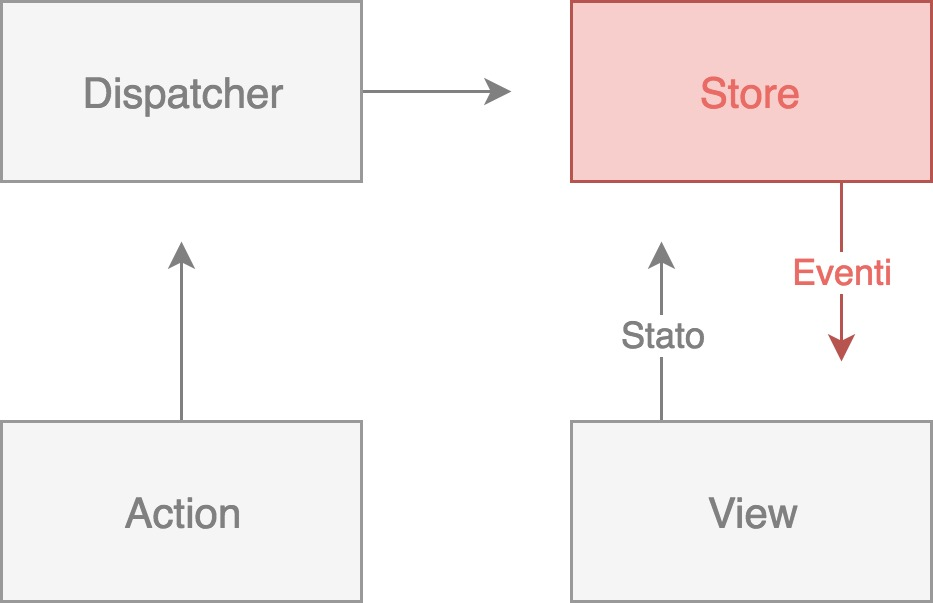
\includegraphics[width=6.5cm]{./images/StoreWorkflow}
\caption{Compiti dello Store nell'architettura Flux.}
\label{StoreWorkflow}
\vspace*{0.5cm} 
\end{figure}

\noindent
Un punto fondamentale riguardo gli Stores è che essi non ricevono modifiche esterne. Tutta la logica relativa al cambiamento dello stato dell'applicazione è contenuta al loro interno e questo semplifica enormemente il lavoro di debugging del codice e rafforza la consistenza dello stato.

\subsubsection*{View}
La View è formata da componenti React strutturati presumibilmente con il pattern spiegato nella Sezione \ref{ReactExplanation}, dei componenti contenitori e di presentazione. Nel caso di Flux, i componenti contenitori sono posizionati al livello più alto ed interagiscono direttamente con gli Store, rimanendo in ascolto dei loro eventi e ottenendo da essi i dati che verranno poi passati ai componenti di presentazione figli.
Utilizzando questa strategia si assicura un corretto flusso dei dati, in cui l'unico punto di ingresso è il componente contenitore all'inizio della catena.

\subsection{Analisi dell'applicazione}
\label{FluxApplication}
Per avere un esempio pratico di questa architettura verrà implementata di nuovo l'applicazione presentata nella Sezione \ref{ExampleApplicationMVC}, questa volta attraverso React e Flux.
In questo caso oltre che la normale sintassi di ES6 c'è anche bisogno di compilare il codice JSX all'interno di questa in modo da ottenere i componenti React desiderati, per questo motivo verrà utilizzato anche il plugin di Babel \textit{React Preset}\footnote{https://babeljs.io/docs/plugins/preset-react}.
Vengono utilizzati due tipi di configurazioni per Webpack: \mintinline{text}{webpack.dev.js} in fase di development, più veloce ma che genera un codice non ottimizzato; \mintinline{text}{webpack.prod.js} in fase di produzione, più lenta che genera però un codice più leggero e veloce.

Il codice dell'applicazione è diviso in due parti principali: i componenti React nella cartella \mintinline{text}{flux/src/components} e gli elementi dell'architettura Flux nella cartella \mintinline{text}{flux/src/data}. Di seguito verranno spiegate in dettaglio queste due parti.

\subsubsection*{I componenti React}
Il componente più ad alto livello, in cui viene inizializzata l'applicazione, e dove React viene aggiunto materialmente al DOM è situato in \mintinline{text}{flux/src/app.js}. Salta subito all'occhio che questo è un componente “di passaggio” ed utilizzato solo per inizializzare React. Il vero e proprio componente più ad alto livello, e che possiamo considerare come componente “container” è \mintinline{text}{flux/src/components/Bookshelf.js}.

\begin{listing}[ht]
\inputminted{javascript}{sources/applicationFluxBookshelfState.js}
\caption{Esempio di interazione tra componente container e Store.} 
\label{applicationFluxBookshelfState} 
\end{listing} 

\noindent
Il Codice \ref{applicationFluxBookshelfState} rappresenta l'interazione tra il componente container Bookshelf e lo Store principale dell'applicazione. Questa interazione si divide in due parti:

\begin{enumerate}
    \item Nel costruttore viene inizializzato lo stato del componente ottenendolo dallo Store tramite il metodo \mintinline{text}{BookshelfStore.getBooks()}.

    \item Nel metodo \mintinline{text}{componentWillMount()}, che React esegue automaticamente durante l'inizializzazione del componente, viene iniziato l'ascolto dell'evento di aggiornamento dello Store assegnandolo alla funzione interna \mintinline{text}{_onChange()} che provvederà a sincronizzare lo stato del componente con quello dello Store.
\end{enumerate}

\noindent
Il componente container ha poi il compito di comporre l'interfaccia utilizzando gli altri componenti di presentazione a disposizione, e passare loro i dati e le funzioni per il corretto funzionamento dell'applicazione.

\begin{listing}[ht]
\inputminted{jsx}{sources/applicationFluxBookshelfRender.js}
\caption{Esempio di composizione tra componente container e di presentazione.} 
\label{applicationFluxBookshelfRender} 
\end{listing} 

\noindent
Nel Codice \ref{applicationFluxBookshelfRender} viene utilizzato il componente \mintinline{text}{<AddBook />} definito all'interno del file \mintinline{text}{AddBook.js}, al quale viene passata la funzione \mintinline{text}{_handleAddBook(title, author)} che gestirà l'evento di aggiunta di un nuovo libro emanando l'Action relativa al Dispatcher. Tutti i componenti di presentazione utilizzati per comporre l'interfaccia sono dipendenti dal componente container \mintinline{text}{<Bookshelf />} e non comunicano direttamente con l'architettura Flux. Un componente di presentazione è solitamente composto solamente da una funzione che ritorna codice JSX in base alle proprietà ricevute dal componente superiore.

\begin{listing}[ht]
\inputminted{jsx}{sources/applicationFluxButton.js}
\caption{Esempio di un semplice componente di presentazione.} 
\label{applicationFluxButton} 
\end{listing} 

\noindent
Ad esempio questo componente, che rappresenta un semplice bottone, è riutilizzabile all'interno dell'applicazione in quanto a seconda del contesto possiamo cambiare il suo contenuto e comportamento a seconda delle proprietà passate.

E' possibile creare un componente contenitore all'interno di un altro, se è necessario gestire elementi dell'interfaccia piuttosto complessi. Questo è il caso del componente \mintinline{text}{<AddBook />}, che rappresenta il form di aggiunta di un nuovo libro, composto dai vari campi di testo ed il bottone di invio, e mantiene al suo interno lo stato di questi vari elementi. È bene prestare attenzione nell'aggiungere componenti contenitori nidificati, sopratutto nel non utilizzarli per interagire con l'architettura, compito che dovrebbe essere lasciato sempre al componente di più alto livello.

\subsubsection*{La gestione dei dati}
L'architettura Flux è implementata attraverso i componenti presenti nella cartella \mintinline{text}{flux/src/data}. Il primo file da analizzare è \mintinline{text}{BookshelfActions.js}, una libreria che fornisce le Actions eseguibili all'interno dell'applicazione sotto forma di funzione, e le fa emettere direttamente dal Dispatcher. Questo tipo di utility è comunemente chiamata in ambito Flux: \textit{ActionCreator}.

\begin{listing}[ht]
\inputminted{jsx}{sources/applicationFluxActions.js}
\caption{Esempio di ActionCreator dell'applicazione.} 
\label{applicationFluxActions} 
\end{listing} 

\noindent
Nell'esempio del Codice \ref{applicationFluxActions} viene riportata una funzione che automatizza l'emissione dell'azione \mintinline{text}{ADD_BOOK} al Dispatcher, fornendo come payload il titolo e l'autore del libro.
Le funzioni implementate dall'ActionCreator vengono generalmente utilizzate dal componente container per interagire in maniera corretta con lo Store.

Le Action devono essere emesse dal Dispatcher, questo nell'applicazione viene implementato nel file \mintinline{text}{BookshelfDispatcher.js} utilizzando quello messo a disposizione automaticamente dalla libreria \textit{Flux}. Questo Dispatcher, implementato ed attualmente utilizzato anche da Facebook, è una versione molto più potente del codice esempio esposto nella Sezione \ref{FluxComponents}.

\begin{listing}[ht]
\inputminted{jsx}{sources/applicationFluxDispatcher.js}
\caption{Dispatcher dell'applicazione.} 
\label{applicationFluxDispatcher} 
\end{listing} 

\noindent
Viene esportata direttamente un'istanza che ci fornisce un singleton, in quanto il Dispatcher deve essere unico all'interno dell'applicazione e condiviso tra tutti i componenti che hanno bisogno di effettuare azioni.

L'ultimo componente che viene preso in esame è lo Store, implementato nel file \mintinline{text}{BookshelfStore.js}. Questo ha il compito di gestire lo stato dell'applicazione mantenendo una lista di libri in \mintinline{text}{this.state}, pre-popolata attraverso il file JSON \mintinline{text}{db.json}, e anche quello di fornire al Dispatcher la funzione incaricata di gestire le Action emesse.

\begin{listing}[ht]
\inputminted{jsx}{sources/applicationFluxStore.js}
\caption{Registrazione dello Store nel Dispatcher} 
\label{applicationFluxStore} 
\end{listing}

\noindent
Analizzando il Codice \ref{applicationFluxStore} è possibile notare che lo Store viene creato estendendo la classe \mintinline{text}{EventEmitter}, questo perché ogni Store ha la necessità di mandare eventi all'interno dell'applicazione ogni qualvolta lo stato viene modificato. Troviamo poi all'interno del costruttore della classe il metodo \mintinline{text}{BookshelfDispatcher.register()} che prende come parametro la funzione dello Store da registrare nel Dispatcher. La funzione che verrà aggiunta è \mintinline{text}{_registerActions()} la quale prende come parametro un'Action e, come da prassi, la getta in pasto ad un costrutto \mintinline{text}{Switch} che la eseguirà sullo Store corrente.


\subsection{Flux ed il flusso dei dati}
Come possiamo notare dalla Sezione \ref{FluxApplication}, l'architettura di Flux rispetto a quella MVC è molto più strutturata, ed i dati e gli eventi devono sottostare a delle regole e dei percorsi più rigidi, cosa che permette di avere un maggiore controllo sui comportamenti dell'applicazione e sui cambiamento dello stato. In Flux gli effetti collaterali derivati dall'aggiornamento dello stato sono molto facili da controllare, e grazie alla rigidità dell'architettura anche in numero molto inferiore. Quando uno Store riceve un'Action, ed il suo stato viene modificato, emette un evento grazie al quale le View dell'applicazione si modificheranno di conseguenza. Questo è l'unico, ed inevitabile, caso in cui la modifica dello stato causa un'ulteriore esecuzione di codice. 
Tuttavia il vantaggio di Flux non sta solo in questo, ma anche nel gestire in modo chiaro (Ma non perfetto, come vedremo nella Sezione \ref{ReduxArchitecture}) le dipendenze tra due Store differenti. In un'architettura MV* non esiste un vero e proprio approccio che permette di eseguire un cambiamento solo se ne è stato fatto un'altro in precedenza, se non in maniera imperativa e notificando manualmente il componente dipendente. In Flux questo problema è risolto semplicemente dichiarando la dipendenza all'interno dello Store tramite la funzione \mintinline{text}{Dispatcher.waitFor()} descritta nella Sezione \ref{FluxComponents}.
Un altro elemento a favore di Flux riguarda sempre lo Store e come questo integri in se stesso tutti i possibili cambiamenti che lo stato possa fare. Ciò fa sì che nel caso in cui si debba analizzare un certo cambiamento, la sua posizione all'interno del codice sia immediata. Questo impedisce la creazione di cambi di stato nascosti o non previsti, classici durante lo sviluppo di applicazioni MV* \cite{boduch2016flux}.

Tutto ciò espresso fino ad ora è indubbiamente un punto a favore a livello di architettura, di gestione dei dati e degli eventi, tuttavia a livello implementativo possono sorgere dei difetti non trascurabili.
In Flux lo Store notifica le View del cambiamento del proprio stato, senza specificare cosa è stato cambiato come ad esempio potrebbe capitare in altre architetture. Questo comporta un lavoro più oneroso da parte della View, la quale potrebbe dover aggiornare, anche inutilmente, più componenti del necessario. Proprio per questo motivo React è considerato un'ottima libreria per Flux in quanto riesce ad aggiornare solamente il DOM che viene effettivamente modificato.
Un'altra problematica sempre riguardo gli Store è quando il loro numero e la loro complessità diventa elevata, e di conseguenza diventa molto difficile gestire le dipendenze delle Action nonostante la presenza del Dispatcher. Queste dipendenze possono diventare sempre più numerose, complesse e difficili da gestire all'aumentare del numero di features dell'applicazione.
Un altro punto a sfavore di Flux riguarda le Action. Ogni cosa che accade all'interno dell'applicazione deve essere descritta con un'Action, ed facile immaginare che una singola feature può dunque crearne un numero non irrilevante. Tenere traccia di ognuna di esse diventa quindi un compito non proprio semplice nonostante l'aiuto di una libreria ActionCreator.

\section{Architettura Redux}
\label{ReduxArchitecture}